In this chapter we will begin reviewing the theories that are involved in a two-photon process. Two-photon processes come about through second-order perturbation theory so a brief description of it will allow for a greater understanding of the topic as a whole. We will be looking at how photons interact with matter to develop the operator we will be using in this study. From there we will be reviewing how time-orderings of the two photons is involved as well as how the basic theory works overall. This chapter will also discuss our results and derivation of the two-photon decay rate, how it relates to its two-photon Einstein B absorption coefficient and the results of it being applied to astrophysics. In addition to this we will be going over how it can be applied to Raman scattering as well as a brief discussion of how Raman and Rayleigh scattering differ from each other and other two-photon processes. Finally we will be presenting our results of all of these calculated values as they are scaled up through heavier hydrogenlike ions. 
\section{Second-Order Perturbation Theory}
Before discussing two-photon processes we must first discuss its root, being second-order perturbation theory. To begin we split up our Hamiltonian into two parts being \cite{variational}
\begin{equation}
\mathscr{H}=\mathscr{H}_0+\lambda\mathscr{H}_1
\end{equation}
where $\mathscr{H}_0$ is our unperturbed Hamiltonian which can be solved for analytically, and $V$ is our perturbation which is controlled by the parameter $\lambda$. We then expand our wave equations and energies in terms of our scale factor $\lambda$
\begin{equation}
    \begin{split}
        \Psi&=\Psi_0+\lambda\Psi_1+\lambda^2 \Psi_2\\
        E&=E_0+\lambda E_1+ \lambda^2 E_2
    \end{split}
\end{equation}
First-order perturbation was derived in a previous section so we will only focus on second-order perturbation here. Solving for the second order correction to the energy we have
\begin{equation}
    E_2=\frac{1}{\braket{\Psi_0}{\Psi_0}} \left[ 2\bra{\Psi_0}V\ket{\Psi_1}+2\bra{\Psi_0}H_0-E_0\ket{\Psi_2}+\bra{\Psi_1}H_0-E_0\ket{\Psi_1}\right]
\end{equation}
This is formed from terms with $\lambda^2$. $E_2$ is stable with respect to variations of $\Psi_2$, the second-order perturbation equation is
\begin{equation}
    (\mathscr{H}_0-E_0)\ket{\Psi_2}+ (V-E_1)\ket{\Psi_1}=E_2\ket{\Psi_0}
\end{equation}
then it follows that
\begin{equation}
    E_2=\frac{\bra{\Psi_0}V-E_1\ket{\Psi_1}}{\braket{\Psi_0}{\Psi_0}}
\end{equation}
and using the definition of $\Psi_1$ if it satisfies the first-order perturbation equation
\begin{equation}
    \ket{\Psi_1}= \frac{-(V-E_1)\ket{\Psi_0}}{H_0-E_0}
\end{equation}
we then multiply by unity 
\begin{equation}
    1=\int\sum_{n=1}^\infty \ket{\Psi n}\bra{\Psi n}
\end{equation}
to get our first-order perturbation to the wave equation as
\begin{equation}
    \ket{\Psi_1}=\int\sum_{n=1}^\infty \frac{\ket{\Psi n}\bra{\Psi n} -(V-E_1)\ket{\Psi_0}}{E_0 n-E_0}
\end{equation}
which we then substitute into our second-order perturbation to the energy to give
\begin{equation}
    E_2=\int\sum_{n=1}^\infty \frac{\bra{\Psi_0}V-E_1\ket{\Psi n}\bra{\Psi n} -(V-E_1)\ket{\Psi_0}}{E_0 n-E_0}
\end{equation}
For the particular case of solving the dipole polarizability for the s-state we use the fact that $E_1=0$ for the operator used is $V=Fr\cos{\theta}$. As detailed in previous sections we use a discrete basis set to represent the intermediate states, rather than summing over the entire spectrum and integrating over the continuum. The purpose of this derivation will be made obvious in the following sections, as the equation for the second-order perturbation is extremely similar to the matrix elements of a two-photon transition.

\section{Single-Photon Transitions}
In this section we will detail the derivation of the form of the interaction operator that we will be using in our two-photon transition. We first start from the definition of the Hamiltonian
\begin{equation}
    \mathscr{H}=\frac{p^2}{2m}+V
\end{equation}
through which we make the transformation to the canonical momentum
\begin{equation}
    \Vec{p}\rightarrow \Vec{p}-\frac{e}{c}\Vec{A}
\end{equation}
the Hamiltonian then becomes
\begin{equation}
    \begin{split}
            \mathscr{H}&=\frac{(\Vec{p}-\frac{e}{c}\Vec{A})^2}{2m}+V\\
            &=\frac{p^2}{2m}-\frac{e}{2mc}\Vec{p}\cdot\Vec{A}+\frac{e}{2mc}\Vec{A}\cdot\Vec{p}+\frac{e^2}{2mc^2}\Vec{A}^2+V
    \end{split}
\end{equation}
where
\begin{equation}
    \Vec{A}=A_0 \hat{e}e^{i\Vec{k}\cdot\Vec{r}-i\omega t}
\end{equation}
is the vector potential for a plane wave. Using the definition of a plane wave
\begin{equation}
    \abs{\Vec{k}}=\omega/c
\end{equation}
being of order $\alpha=1/c$ in atomic units and
\begin{equation}
    \Vec{k}\cdot\hat{e}=0
\end{equation}
for a transverse wave, we expand the Hamiltonian as
\begin{equation}
    \mathscr{H}= \frac{p^2}{2m}-\frac{2eA_0}{2mc}\Vec{p}\cdot\hat{e}[1-i\Vec{k}\cdot\Vec{r}+\cdots]e^{-i\omega t}
\end{equation}
Keeping only the first order term and using the fact that $\nabla\cdot A=0$ for a transverse wave we have
\begin{equation}
    \mathscr{H}_1=-\frac{eA_0}{2mc}2\Vec{p}\cdot\hat{e}
\end{equation}
We then calculate the transition matrix elements
\begin{equation}
    \bra{\Psi_i}\mathscr{H}_1\ket{\Psi_f}=\bra{\Psi_i}\Vec{p}\cdot\hat{e}\ket{\Psi_f}
\end{equation}
and use the commutator relation to get the operator into length form where
\begin{equation}
   \frac{m}{\hbar} \bra{\Psi_i}[\mathscr{H},\Vec{r}\cdot\hat{e}]\ket{\Psi_f}=\frac{m}{\hbar}(E_i-E_f)\bra{\Psi_i}\Vec{r}\cdot\hat{e}\ket{\Psi_f}
\end{equation}
This is the form of the interaction operator used in the next section for the two-photon transitions that are being studied. From this we can also show how energy is conserved. Using definitions for the time dependent portion of the wave equations where
\begin{equation}
    \Psi_i=e^{-iE_i t/\hbar}
\end{equation}
and
\begin{equation}
    \Psi_f=e^{-iE_f t/\hbar}
\end{equation}
This leads to the time integral
\begin{equation}
    \int_0^\infty(e^{-iE_i t/\hbar})^* e^{-i\omega t}e^{-iE_f  t/\hbar}dt=2\pi\delta\left(\frac{E_i}{\hbar}-\omega-\frac{E_f}{\hbar}\right)
\end{equation}
which leads to the conservation of energy relation
\begin{equation}
    \omega=(E_i-E_f)\hbar
\end{equation}
\section{Two-Photon Transitions}
Two-photon transitions come about through second-order perturbation theory \cite{loudon}. % with the second order perturbation taking the form of either \cite{mizushima1970quantum}
%\begin{equation}
%    P_{i\rightarrow f}=\frac{2\pi}{\hbar^2}\abs{\bra{f}\mathscr{H}\ket{i}}^2\delta(\omega_{if%})
%\end{equation}
%or
%\begin{equation}
%    P_{i\rightarrow f}=\frac{2\pi}{\hbar^2}
%    \abs{\frac{\bra{f}\mathscr{H}\ket{n}\bra{n}\mathscr{H}\ket{i}}
%    {\bra{n}\mathscr{H}\ket{n}-\bra{i}\mathscr{H}\ket{i}}}^2\delta(\omega_{if}).
%\end{equation}
%With $i$ and $f$ representing the initial and final states respectively, and $\omega_{if}$ representing the transition energy between the initial and final states.
%The first case is negligible due to both photons being absorbed by the system at the exact same time being a second order correction which has a much lower magnitude.The second scenario is far more probable as it is a first order correction and is what will be used in the analysis going forward.
The hyperfine transition that is being studied is a two-photon process where the transition from the ground state to the excited state is mediated by a transition to an intermediate virtual state $\ket{n}$ .These two photons can have any frequency $\omega$ so long as the sum of their energies $\hbar \omega_1+\hbar \omega_2$ is equal to the total transition energy.
\begin{center}

        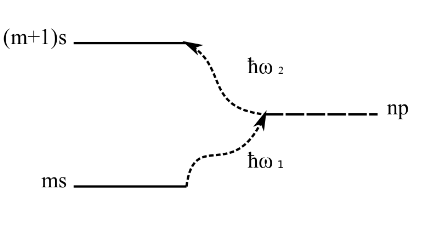
\includegraphics[width=0.4\textwidth]{images/transitioncrop.PNG}

\end{center}
The most probable atomic transitions involve emission or absorption of a single photon, where an atom starts in an initial state and then either absorbs or emits a single photon to go into either a higher or lower state respectively. We can represent this transition in bra-ket notation with the initial state $\ket{i}$ being operated on by the dipole operator \(\hat{e}\cdotp\Vec{r}\) to arrive at our final state $\ket{f}$. The dipole matrix element is then
\begin{equation}
    \bra{f}\hat{e}\cdotp\Vec{r}\ket{i}
\end{equation}
The construction of a two-photon transition is very similar. The major difference being that there is an intermediate virtual state in between the initial and final states. Starting with the initial state $\ket{i}$, operated on by \(\hat{\epsilon}\cdotp\Vec{r}\) to go to an intermediate virtual state $\bra{n}$. A second transition is then done by operating on the intermediate virtual state with \(\hat{\epsilon}\cdotp\Vec{r}\) to excite to the final state $\bra{f}$.
\begin{equation}
        \bra{f}\hat{e}\cdotp\Vec{r}\ket{n}\bra{n}\hat{e}\cdotp\Vec{r}\ket{i}
\end{equation}
The energies of the two photons do not have to be identical. The only constraint on them is that the sum of their energies must equal the transition energy from the initial state to the final state, due to conservation of energy. This brings up a unique problem in that the photons are not indistinguishable from each other. So the order in which the photons interact with the atom matter, and we must consider the three possible time-orderings that can occur.
\begin{figure}
    \centering
    \caption{Time orderings of a two-photon process}
    \label{fig:Timeorder}
    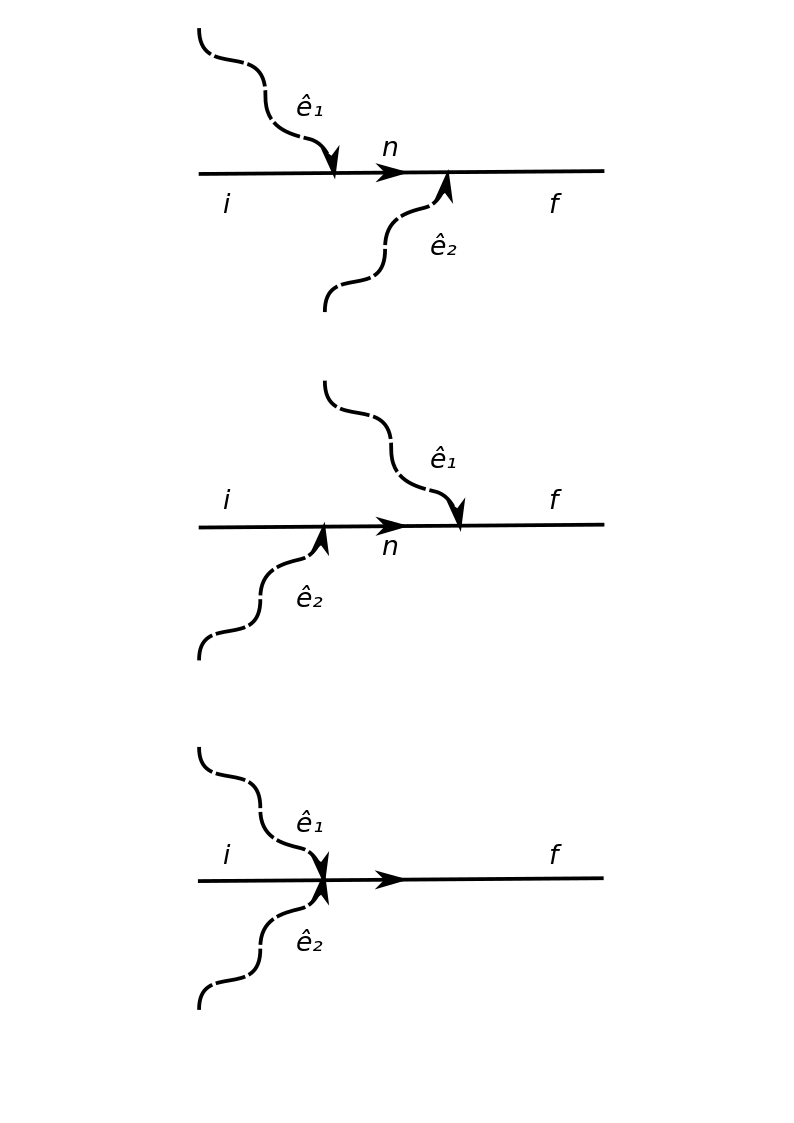
\includegraphics[width=0.4\textwidth]{images/twopproc.png}
\end{figure}

When talking about the different time-orderings in which two-photon processes can occur. it is assumed that the process happens instantly. The first time ordering shows the atom absorbing the first photon \(\hat{e}_1\), jumping to an intermediate state, absorbing the second photon \(\hat{e}_2\) and jumping to the final state. The second time ordering shows the same process except the order of the photons is reversed. The final time ordering shows both of the photons being absorbed simultaneously, this is a second order term and is therefore far less probable. The equation now changes to account for the specific order that the two photons are absorbed so that we average over the two time-orderings.
\begin{equation}
        \abs{
        \bra{f}\hat{e}_2\cdotp\Vec{r}\ket{n}
        \bra{n}\hat{e}_1\cdotp\Vec{r}\ket{i}
        +
        \bra{f}\hat{e}_1\cdotp\Vec{r}\ket{n}
        \bra{n}\hat{e}_2\cdotp\Vec{r}\ket{i}
        }^{2}
\end{equation}
We will specifically be considering a \(1s\) to \(2s\) transition in hydrogen using two photons. This transition is unique due to the the stability of the \(2s\) state giving rise to a lifetime of \(0.125\) s \cite{lifetime}, which is a tremendously long lifetime compared to other states. Due to parity, this transition can only occur through a two-photon decay so it is ideal as a demonstration. Using the previously built equations for two-photon processes along with the summation over pseudostates, from the previous chapter, our expression for the matrix elements of this transition is proportional to.
\begin{equation}
    \sum_{n} \abs{
    \frac{\bra{2s}z\ket{n}
    \bra{n}z\ket{1s}}
    {E_{n}-E_{0}+\omega_{1}}+
    \frac{\bra{2s}z\ket{n}
    \bra{n}z\ket{1s}}
    {E_{n}-E_{0}+\omega_{2}}
    }^{2}
\end{equation}
When considering the exchange of angular momentum going from a \(1s\) state where \(l=0\) to a \(2s\) where \(l=0\) the triangular rule tells us that the total angular momentum exchanged is 0. This is relevant due to the fact that each photon carries with it one unit of angular momentum. For this to occur the two photons are antiparallel thus the total angular momentum exchanged sum to zero. From this we calculate a full decay rate
\begin{equation}
    A(\nu_1)d\nu_1=\frac{1024\pi^6 e^4}{\hbar^2 c^4}\nu_1^3\nu_2^3
    \abs{(\hat{e}_1 \cdot \hat{e}_2)}^2
    \abs {\sum_{n} 
    \frac{\bra{2s}z\ket{n}
    \bra{n}z\ket{1s}}
    {E_{n}-E_{0}+\nu_{1}}+
    \frac{\bra{2s}z\ket{n}
    \bra{n}z\ket{1s}}
    {E_{n}-E_{0}+\nu_{2}}
    }^{2}
\end{equation}
with the total decay rate given by
\begin{equation}
    A=\frac{1}{2}\int_0^\nu A(\nu_1)d\nu_1
\end{equation}
where the factor of \(\frac{1}{2}\) is introduced because only unique pairs of photons are to be counted.
Observing the terms in this equations we see that the decay rate will be greatest when \(\omega_1 = \omega_2\) when the polarization of the polarization vectors are parallel or anti-parallel. This however will not be the case when considering this transition between the hyperfine levels being studied.

\section{Applications to Hyperfine Transitions in Hydrogen}
The hyperfine levels in ground-state hydrogen are represented by the eigenvectors
\begin{equation}
    \ket{1slsJIFM_f}
\end{equation}
with $s$ and $l$ representing the electrons spin and orbital angular momentum. These two angular momenta couple together to give the total angular momentum $J$ which is coupled with the spin of the nucleus $I$ to give the quantum number for hyperfine levels $F$. With \(M_f\) being the projection of $F$ onto the z-axis. The hyperfine levels of the ground state are separated into the two levels $F=0$ and $F=1$. Since this is a transition between two $s$ states, single-photon electric-dipole transitions are forbidden due to angular momentum and parity selection rules. Therefore two-photon processes are required. We will specifically be calculating the decay rate and absorption coefficient due to this process and will see if it is a potentially significant correction to astrophysical processes on cosmological distance scales. In addition to this, we will also be calculating cross sections for Raman scattering. For either of these processes we must first calculate the matrix elements using the equation
\begin{equation}
    \mathcal{M}^{-\gamma\gamma}(\hat{e}_i\rightarrow \hat{e}_f)=
    \sum_{n}
    \frac{
    \bra{f}\hat{e}_{2}\cdot
    \Vec{r}\ket{n}
    \bra{n}\hat{e}_{1}\cdot\Vec{r}\ket{i}}
    {\omega_{ni}+\omega_{1}}
    +
    \frac{
    \bra{f}\hat{e}_{1}\cdot\Vec{r}\ket{n}
    \bra{n}\hat{e}_{2}\cdot\Vec{r}\ket{i}}
    {\omega_{ni}+\omega_{2}}
\end{equation}
with both time-orderings of the photons being considered and all polarizations $\hat{e}$ of the two photons being accounted for by the dipole operator \(\hat{e}\cdot\Vec{r}\) where
\begin{equation}
    \hat{e_r}\cdot\Vec{r}= e_0r_0-e_+r_--e_-r_+
\end{equation}
\begin{equation}
    \begin{split}
        r_0&=z\\
        r_{\pm}&=\mp \frac{1}{\sqrt{2}}(x\pm iy)
    \end{split}
\end{equation}
\begin{equation}
    \begin{split}
        e_0&=e_z\\
        e_{\pm}&=\mp \frac{1}{\sqrt{2}}(e_x\pm ie_y)
    \end{split}
\end{equation}
and by conservation of energy
\begin{equation}
    \hbar \omega_1+\hbar \omega_2= E_i -E_f
\end{equation}
Summing this expression over all polarizations gives
\begin{equation}
\begin{split}
    \mathcal{M}^{-\gamma\gamma}(i\rightarrow f)=\\
    \sum_{\mu_1=-1}^1
    \sum_{\mu_2=-1}^1
    \sum_{n}
    (-1)^{\mu_2}(-1)^{\mu_1}
    \frac{
    \bra{f}{e}_{\mu_2}
    {r}_{-\mu_2}\ket{n}
    \bra{n}{e}_{\mu_1}{r}_{-\mu_1}\ket{i}}
    {\omega_{ni}+\omega_{1}}\\
    +(-1)^{\mu_1}(-1)^{\mu_2}
    \frac{
    \bra{f}{e}_{\mu_1}{r}_{-\mu_1}\ket{n}
    \bra{n}{e}_{\mu_2}{r_{-\mu_2}}\ket{i}}
    {\omega_{ni}+\omega_{2}}.
    \end{split}
\end{equation}
We may now include all the relevant quantum numbers for these transitions with the corresponding eigenvectors given by
\begin{equation}
    \ket{1s l s J I F M_f}
\end{equation}
for the initial state
\begin{equation}
    \ket{np l's'J'I'F'M_f'}
\end{equation}
as the intermediate state, and
\begin{equation}
        \bra{1s l'' s'' J'' I'' F'' M_f''}
\end{equation}
as the final state.
For the current purposes the only two quantum numbers that matter are the hyperfine splitting quantum number $F$ and its projection \(M_f\). The rest will be written together as \(\gamma\). We must also sum over all possible magnetic quantum numbers for the final states and  over the intermediate states with \(M_f''=-1,0,1\) and \(M_f'=-1,0,1\). Rewriting the transition equations gives us
\begin{equation}
\begin{split}
    \mathcal{M}^{-\gamma\gamma}(F\rightarrow F'')=
    \sum_{M_f''=-1}^1
    \sum_{M_f'=-1}^1
    \sum_{\mu_1=-1}^1
    \sum_{\mu_2=-1}^1
    \sum_{n}\\
    (-1)^{\mu_2}(-1)^{\mu_1}
    \frac{
    \bra{\gamma'' F'' M_F''}{e}_{\mu_2}
    {r}_{-\mu_2}\ket{\gamma' F' M_F'}
    \bra{\gamma' F' M_F'}{e}_{\mu_1}{r}_{-\mu_1}\ket{\gamma F M_F}}
    {\omega_{n0}+\omega_{1}}\\
    +(-1)^{\mu_1}(-1)^{\mu_2}
    \frac{
    \bra{\gamma'' F'' M_F''}{e}_{\mu_1}{r}_{-\mu_1}\ket{\gamma' F' M_F'}
    \bra{\gamma' F' M_F'}{e}_{\mu_2}{r_{-\mu_2}}\ket{\gamma F M_F}}
    {\omega_{n0}+\omega_{2}}.
    \end{split}
\end{equation}
To evaluate these matrix elements we first strip away the dependence on the magnetic quantum numbers by using the Wigner-Eckart theorem to calculate the reduced matrix element \cite{edmonds}
\begin{equation}
    (\gamma'j'm'\abs{T^k_q}\gamma jm)=(-1)^{j-m}
    \begin{pmatrix}
    j'  &k &j \\
    -m' &q &m
    \end{pmatrix}
    (\gamma'j'\abs{\abs{T^k}}\gamma j)
\end{equation}
or in this case
\begin{equation}
    (\gamma'F'M_f'\abs{r_{-\mu}}\gamma FM_F)=(-1)^{F-M_F}
    \begin{pmatrix}
    F'  &1 &F \\
    -M_F' &-\mu &M_F
    \end{pmatrix}
    (\gamma'F'\abs{\abs{r}}\gamma F)
\end{equation}
This changes our equation to
\begin{equation}
\begin{split}
    \mathcal{M}^{-\gamma\gamma}(F\rightarrow F'')=
    -\sqrt{\frac{1}{18}}\sum_{n}\\
    (e_2\cross e_1)
    \frac{
    (\gamma'' F''\abs{\abs{r}}\gamma' F')
    (\gamma' F'\abs{\abs{r}}\gamma F)}
    {\omega_{n0}+\omega_{1}}\\
    +(e_1\cross e_2)
    \frac{
    (\gamma'' F'' \abs{\abs{r}}\gamma' F')
    (\gamma' F'\abs{\abs{r}}\gamma F)}
    {\omega_{n0}+\omega_{2}}.
    \end{split}
\end{equation}
Using the fact that
\begin{equation}
    (e_1\cross e_2)=-(e_2\cross e_1)
\end{equation}
and that we must now strip away the dependence on the coupling of the total angular momentum with the spin of the nucleus we rewrite our equation as
\begin{equation}
\begin{split}
    \mathcal{M}^{-\gamma\gamma}(F\rightarrow F'')=
    -\sqrt{\frac{1}{18}} (e_2\cross e_1)\sum_{n}\sum_{J'=1/2}^{3/2}\\
    \frac{
    (\gamma''J''I'' F''\abs{\abs{r}}\gamma'J'I' F')
    (\gamma'J'I' F'\abs{\abs{r}}\gamma JI F)}
    {\omega_{n0}+\omega_{1}}\\
    -
    \frac{
    (\gamma''J''I'' F'' \abs{\abs{r}}\gamma'J'I' F')
    (\gamma'J'I' F'\abs{\abs{r}}\gamma JI F)}
    {\omega_{n0}+\omega_{2}}.
    \end{split}
\end{equation}
It is significant that as in the case of triplet helium decay \cite{dalgarnohelium} where one unit of angular momentum is exchanged in a two-photon process, the matrix element is proportional to the cross product of the polarization vectors, leading to a minus sign between the two terms. We now use the definition of a $6j$ symbol for two coupled angular momenta \cite{edmonds7}
\begin{equation}
\begin{split}
        (\gamma'j_1'j_2J'\abs{\abs{T(k)}}\gamma j_1 j_2 J)\\
        =(-1)^{j_1'+j_2+J+k}[(2J+1)(2J'+1)]^{\frac{1}{2}}
        \begin{Bmatrix}
        j_1' & J'  &j_2\\
        J    & j_1 &k
        \end{Bmatrix}
        (\gamma' j_1'\abs{\abs{T(k)}}\gamma j_1)
\end{split}
\end{equation}
In using this equation, we must take into consideration the fine structure splitting between the $J'=\frac{1}{2}$ and $J'=\frac{3}{2}$ p-states in hydrogen. Otherwise the two contributions cancel exactly. In addition to this we will apply the definition of the $6j$ symbol twice. First stripping away the dependence on the spin of the nucleus and second to strip away the dependence on the spin of the electron. This will give us a completely reduced matrix element
\begin{equation}
\begin{split}
    \mathcal{M}^{-\gamma\gamma}(i\rightarrow f)=
    \frac{1}{9}(e_2\cross e_1)
    \sum_{n}\\
    \frac{
    (1s\abs{\abs{r}}np)(np\abs{\abs{r}}1s)}     {\omega_{n_{\frac{3}{2}}0}+\omega_{1}}
    +
    \frac{
    (1s\abs{\abs{r}}np)(np\abs{\abs{r}}1s) }    {\omega_{n_{\frac{1}{2}}0}+\omega_{2}}\\
    -
    \frac{
    (1s\abs{\abs{r}}np)(np\abs{\abs{r}}1s) }    {\omega_{n_{\frac{1}{2}}0}+\omega_{1}}
    -
    \frac{
    (1s\abs{\abs{r}}np)(np\abs{\abs{r}}1s) }    {\omega_{n_{\frac{3}{2}}0}+\omega_{2}}
    \end{split}
\end{equation}
From here we can use the Wigner-Eckart theorem for $3j$ symbols to calculate the reduced matrix element
\begin{equation}
    (\gamma'j'\abs{\abs{T(k)}}\gamma j)=
    \frac{(\gamma'j'm'\abs{T(kq)}\gamma j m)}
    {
    (-1)^{j'-m'}
    \begin{pmatrix}
    j'  &k  &j\\
    -m' &q  &m
    \end{pmatrix}
    }
\end{equation}
For this we use the $z$ operator and \(m_l=0\) for the magnetic quantum numbers as it is convenient to calculate analytically. This changes the resulting equation to
\begin{equation}
\begin{split}
    \mathcal{M}^{-\gamma\gamma}(i\rightarrow f)=
    -\frac{1}{3}(e_2\cross e_1)
    \sum_{n}\bra{1s}z\ket{np}\bra{np}z\ket{1s}\\
    \bigg(
    \frac{1}{\omega_{p_{\frac{3}{2}}0}+\omega_{1}}
    +
    \frac{1} {\omega_{p_{\frac{1}{2}}0}+\omega_{2}}
    -
    \frac{1} {\omega_{p_{\frac{1}{2}}0}+\omega_{1}}
    -
    \frac{1} {\omega_{p_{\frac{3}{2}}0}+\omega_{2}}
    \bigg)
    \end{split}
\end{equation}
To display explicitly the difference between the $J'=\frac{1}{2}$ and $J'=\frac{3}{2}$ p-states, we find a common denominator. We also take the approximation that the fine structure splitting is relatively small compared to the other energy terms
\begin{equation}
     \frac{1}{\omega_{p_{\frac{3}{2}}0}+\omega}
     - \frac{1} {\omega_{p_{\frac{1}{2}}0}+\omega}
     =\frac{\omega_{3/2-1/2}}{\omega_{p0}^2+2\omega_{p0}\omega+\omega^2}
\end{equation}
where $\omega_{3/2-1/2}=\omega_{p_{\frac{3}{2}}0}-\omega_{p_{\frac{1}{2}}0}$ is the fine structure splitting. Some difficulty comes from calculating this value for a variational basis set. We use the equation for calculating the fine structure energy shift \cite{bethe}
\begin{equation}
    W_1=-\frac{\alpha^2Z^4}{2n^3}\left(\frac{1}{j+\frac{1}{2}}-\frac{3}{4n}\right)
\end{equation}
and evaluate the difference between two states where $j= \frac{3}{2}$ and $j=\frac{1}{2}$, we have the expression
\begin{equation}
    \omega_{p\frac{3}{2}-p\frac{1}{2}}=\frac{\alpha^2Z^4}{4n^3}
\end{equation}

Taking this into account and also considering the fact that the matrix elements are real numbers, the equation becomes 
\begin{equation}
\begin{split}
\mathcal{M}^{-\gamma\gamma}(i\rightarrow f)=
    -\frac{1}{3}(e_2\cross e_1)
    \sum_{n}\bra{np}z\ket{1s}^2\\
    \bigg(
    \frac{\omega_{3/2-1/2}}{\omega_{p0}^2+2\omega_{p0}\omega_1+\omega_1^2}
    -\frac{\omega_{3/2-1/2}}{\omega_{p0}^2+2\omega_{p0}\omega_2+\omega_2^2}
    \bigg)
    \end{split}
\end{equation}
which gives the final form for the matrix elements that will be used in the calculation of the decay rate, the absorption coefficient, and the Raman scattering cross section. We calculate this using a variational intermediate basis set with results being in Fig.\ref{fig:Calculation of the Transition Integrals}. As can be seen in the graph, the transition integral becomes zero when the frequencies of the two photons are equal.
\begin{figure}
    \centering
    \caption{Calculation of the transition integrals $\abs{\mathcal{M}^{-\gamma\gamma}(i\rightarrow f)}^2$}
    \label{fig:Calculation of the Transition Integrals}
\begin{tikzpicture}
\begin{axis}[ymin = 0, xlabel= $\omega/\Delta E$, ylabel=$\abs{\mathcal{M}^{-\gamma\gamma}(i\rightarrow f)}^2$, xmin=0, xmax=1, width=13cm,
height=10cm]
\addplot[
color = black,
mark = none] table {FancyM.txt};
\end{axis}
\end{tikzpicture}
\end{figure}
We will first apply this to the calculation of the decay rate using the equation \cite{dalgarnohelium}
\begin{equation}
    A(\nu_1)=\frac{1024\pi^6e^4}{h^2c^6}\nu_1^3\nu_2^3\abs{\mathcal{M}^{-\gamma\gamma}(i\rightarrow f)}^2
\end{equation}
which we change over to a form better suited for the program that we use, that form being as a relation of angular frequency $\omega$
\begin{equation}
     A(\omega_1)=\frac{16e^4}{c^6}\omega_1^3\omega_2^3\abs{\mathcal{M}^{-\gamma\gamma}(i\rightarrow f)}^2
\end{equation}
The evaluation of this function can be seen in Fig.\ref{fig:Calculation of the Decay Rate}.
\begin{figure}
    \centering
    \caption{Calculation of the decay rate A($\omega$)}
    \label{fig:Calculation of the Decay Rate}
\begin{tikzpicture}
\begin{axis}[ymin = 0, xlabel=$\omega/\Delta E$, ylabel= Decay Rate A($\omega$), xmin=0, xmax=1, width=13cm,
height=10cm]
\addplot[
color = black,
mark = none] table {Decay.txt};
\end{axis}
\end{tikzpicture}
\end{figure}
This equation must be integrated over all possible values for \(\omega\) to arrive at the full decay rate.
Due to the fact that
\begin{equation}
    \omega_2=\Delta E_{F=0 \rightarrow F=1}-\omega_1
\end{equation}
the double integration over $\omega_1$ and $\omega_2$ reduces to a single integral over $\omega_1$. In addition to this, due to the symmetric distribution about the mid point $\omega_1 = \omega_2$, we need only account for half of the total integral. This leaves us with the integral.
\begin{equation}
    A=\int_0^{\Delta E_{F=0 \rightarrow F=1}} A(\omega_1) d\omega_1
\end{equation}
which we integrate using the trapezoidal rule. This leads us to the result of
\begin{equation}
    A=1.97(3)\cross10^{-69}\rm{s}^{-1}
\end{equation}
which is an extremely small value. This value however is several orders of magnitude larger than the value calculated by V. P. Demidov. He approximated the value of this transition to be $7.6\cross10^{-73}\rm{s}^{-1}$ \cite{demidov1962two}. The stability of excited hyperfine ground state hydrogen leads to a lifetime of several million years in the single magnetic photon case \cite{lifetime}, but in this case it is several orders of magnitude greater than that. The stability of the calculation can be seen in Fig.\ref{fig:Calculation of the Decay Rate Variational} where it can be seen that the expression converges to an upper bound of the true value as the basis set is enlarged. For the polarizability we can represent the entire spectrum of hydrogen with a two-dimensional basis set. However in this case we need a much larger basis set due to the fine structure energy splitting being dependent on the basis set size.
\begin{figure}
    \centering
    \caption{Calculation of the decay rate A}
    \label{fig:Calculation of the Decay Rate Variational}
\begin{tikzpicture}
\begin{axis}[xlabel=Dimension of Basis set, ylabel= Decay Rate A, width=13cm,
height=10cm]
\addplot[
color = black,
mark = none] table {DecVar.txt};
\end{axis}
\end{tikzpicture}
\end{figure}

To acquire the absorption coefficient from this we must derive it using the Einstein A and B coefficients. This is done in a manner very similar to Woodgate's for the derivation of the Einstein A and B coefficients for a single-photon transition \cite{woodgate1}. We start from the loss rate $D$ and gain rate $N$ of the system \cite{Dehli}.
\begin{equation}
    \begin{split}
        D&=A+B_{22}\rho_1\rho_2+B_{21}\rho_2+B_{12}\rho_1\\
        N&=B_{11}\rho_1\rho_2\\
        \rho_i&= \left(\frac{8\pi h}{c^3}\right)(e^{h\nu_i/kT}-1)\nu_i^3
    \end{split}
\end{equation}
where $A$ is the spontaneous decay rate, $B_{22}$ is the doubly stimulated decay rate, $B_{12}$ and $B_{21}$ are the singly stimulated decay rates for the two separate photon orders and $B_{11}$ is the absorption coefficient. We then proceed to rearrange to get the absorption coefficient in terms of the decay rate
\begin{equation}
    \begin{split}
        \frac{N}{D}&=\left(\frac{A}{\rho_1 \rho_2} +B_{22}+\frac{B_{21}}{\rho_1}+\frac{B_{12}}{\rho_2}\right)^{-1}B_{11}\\
        &=e^{-\Delta E/kT}\left(\frac{g_2}{g_1}\right)\left(\frac{A}{\rho_1 \rho_2} +B_{22}+\frac{B_{21}}{\rho_1}+\frac{B_{12}}{\rho_2}\right)\\
        &=\left(\frac{c^3}{8\pi h}\right)^2 \frac{A}{\nu_1 ^3 \nu_2^3}+B_{22}+
        \left(\frac{c^3}{8\pi h}\right)\frac{B_{21}}{\nu_1^3}+\left(\frac{c^3}{8\pi h}\right)\frac{B_{12}}{\nu_2^3}\left(e^{h\nu_2 /kT}-1\right)\\
        &=\left(\frac{c^3}{8\pi h}\right)^2\left(e^{-\Delta E/kT} -e^{-h\nu_1 /kT}-e^{h\nu_2 /kT}+1 \right) \frac{A}{\nu_1 ^3 \nu_2^3}+B_{22}\\
        &+\left(\frac{c^3}{8\pi h}\right) \left( e^{h\nu_1 /kT}-1\right)\frac{B_{21}}{\nu_1^3}+\left(\frac{c^3}{8\pi h}\right) \left( e^{-h\nu_1 /kT}-1\right)\frac{B_{12}}{\nu_2^3}
    \end{split}
\end{equation}
we put
\begin{equation}
    \left(\frac{c^3}{8\pi h}\right)\frac{B_{21}}{\nu_1^3} = 
    \left(\frac{c^3}{8\pi h}\right)^2 \frac{A}{\nu_1^3 \nu_2^3}
\end{equation}
and
\begin{equation}
  \left(\frac{c^3}{8\pi h}\right)\frac{B_{12}}{\nu_2^3} = 
    \left(\frac{c^3}{8\pi h}\right)^2 \frac{A}{\nu_1^3 \nu_2^3}  
\end{equation}
then
\begin{equation}
\begin{split}
    B_{22}-\left(\frac{c^3}{8\pi h}\right) \frac{B_{21}}{\nu_1^3} - \left(\frac{c^3}{8\pi h}\right) \frac{B_{12}}{\nu_2^3}&=-\left(\frac{c^3}{8\pi h}\right)^2\frac{A}{\nu_1^3 \nu_2^3}\\
    B_{22}-\left(\frac{c^3}{8\pi h}\right)^2\frac{A}{\nu_1^3 \nu_2^3}-\left(\frac{c^3}{8\pi h}\right)^2\frac{A}{\nu_1^3 \nu_2^3}&=-\left(\frac{c^3}{8\pi h}\right)^2\frac{A}{\nu_1^3 \nu_2^3}
\end{split}
\end{equation}
which leads us to the result
\begin{equation}
    \left(\frac{g_2}{g_1}\right)B_{11}=\left(\frac{c^3}{8\pi h}\right)^2
    \frac{A}{\nu_1^3\nu_2^3}
\end{equation}
\begin{figure}
    \centering
    \caption{Calculation of the absorption coefficient B$_{11}$($\omega$)}
    \label{fig:Calculation of the Absorption Rate}
\begin{tikzpicture}
\begin{axis}[ymin = 0, xlabel=$\omega/\Delta E$, ylabel= Absorption coefficient, xmin=0, xmax=1, width=13cm,
height=10cm]
\addplot[
color = black,
mark = none] table {Absorb.txt};
\end{axis}
\end{tikzpicture}
\end{figure}
This equation along with the one for the decay rate gives an overall expression of
\begin{equation}
     B(\omega_1)=\frac{4\pi^2e^4}{\hbar^2}\abs{\mathcal{M}^{-\gamma\gamma}(i\rightarrow f)}^2
\end{equation}
This, similar to the decay rate gives us the function plotted in Fig.\ref{fig:Calculation of the Absorption Rate}. Using the same procedure of integrating over the bounds of the frequency leads us to an absorption coefficient of
\begin{equation}
    B_{11} = 5.28(4)\cross10^{-7} \rm{m^6 J^{-2} s^{-3}}
\end{equation}
Using this value we can calculate the gain rate of a system for several different scenarios using the expression for the gain rate
\begin{equation}
    N=B_{11}\rho_1\rho_2    
\end{equation}
where
\begin{equation}
    \rho_i=\left(\frac{8\pi h}{c^3}\right)(e^{h\nu_i/kT}-1)^{-1} \nu_i^3
\end{equation}
A logical starting point would be to look at how this transition effects the cosmic microwave background radiation where $T=2.72548\,\rm{K}$. Specifically we can look at individual frequencies for these cases. Due to the restriction that the two frequencies of the absorbed photons must sum up to the transition frequency, when we fix one we therefore fix the other by
\begin{equation}
    \omega_2=\omega_{HFS}-\omega_1
\end{equation}
This however does not remove this fact when we integrate over the frequency range where a delta function is present. When this occurs we simply use the fact that
\begin{equation}
    \int_{-\infty}^\infty f(x) \delta(y-x)dx=f(y)
\end{equation}
so we can simply evaluate our expression at the two frequencies we wish such that the total frequency is still equal to the hyperfine transition energy. This would lead to a total expression for the gain rate of
\begin{equation}
    N=\left(\frac{8\pi h}{c^3}\right)(e^{h\nu_i/kT}-1)^{-1} \nu_1^3
    \left(\frac{8\pi h}{c^3}\right)(e^{h\nu_i/kT}-1)^{-1} \nu_2^3
    \frac{4\pi^2e^4}{\hbar^2}\abs{\mathcal{M}^{-\gamma\gamma}(i\rightarrow f)}^2
\end{equation}
\begin{figure}
    \centering
    \caption{Calculation of the gain rate due to CMB radiation}
    \label{fig:gainrateCMB}
\begin{tikzpicture}
\begin{axis}[ymin = 0, xlabel=$\omega/\Delta E$, ylabel= Gain Rate $s^{-1}$, xmin=0, xmax=1, width=13cm,
height=10cm]
\addplot[
color = black,
mark = none] table {GAINCMB.txt};
\end{axis}
\end{tikzpicture}
\end{figure}
whose values can be seen in Fig.\ref{fig:gainrateCMB}. From this it can be seen that even over millions of years it will not be a significant correction to cosmic microwave background radiation.
\begin{figure}
    \centering
    \caption{Calculation of the gain rate due to CMB radiation and a star}
    \label{fig:gainrateCMBSUN}
\begin{tikzpicture}
\begin{axis}[ymin = 0, xlabel=$\omega/\Delta E$, ylabel= Gain Rate $s^{-1}$, xmin=0, xmax=1, width=13cm,
height=10cm]
\addplot[
color = black,
mark = none] table {GAINRATECMBSUN.txt};
\end{axis}
\end{tikzpicture}
\end{figure}
We can do another example where we consider the first photon coming from a sun-like surface of $T=5800\,\rm{K}$ and the second coming from the cosmic microwave background radiation. We can see the results of this in Fig.\ref{fig:gainrateCMBSUN} and can see that due to the function of the black-body radiation for the sun there is a distinct decrease in value for the second half of the frequencies.
\begin{figure}
    \centering
    \caption{Calculation of the gain rate due to a star}
    \label{fig:gainrateSUNSUN}
\begin{tikzpicture}
\begin{axis}[ymin = 0, xlabel=$\omega/\Delta E$, ylabel= Gain Rate $s^{-1}$, xmin=0, xmax=1, width=13cm,
height=10cm]
\addplot[
color = black,
mark = none] table {GAINRATESUNSUN.txt};
\end{axis}
\end{tikzpicture}
\end{figure}
The last scenario to look at would be assuming both photons come from a star and we can see in Fig.\ref{fig:gainrateSUNSUN} that we gain a significant order of magnitude as the temperature of the black body increases. However even over a cosmological time scale this sort of gain rate would still be very insignificant as a correction. This is logical due to the fact that even at higher temperatures the function for a black body is quite low for the relatively long wavelengths we are looking at.

\section{Raman Scattering}
A natural extension of this project would be to look at the hyperfine transition with respect to a Raman scattering process. Raman scattering was originally one of the first two-photon processes ever discovered and we will be seeing if the cross section is large enough for the hyperfine transition in the $1s$, state that it can be recreated in the lab. One thing worth noting for the transition integrals is the change to the denominator when considering scattering processes. Rayleigh and Raman scattering are two scattering processes that are very similar in nature. They each involve a system absorbing a photon, temporarily exciting to a virtual state and then decaying down to a different state. The main difference between Rayleigh and Raman scattering is that in Rayleigh scattering, when the system decays, it decays to the original state and the photon is of the same frequency as the one that was absorbed. This can be simply stated as Rayleigh scattering being an elastic process. In Raman scattering however the initial and final state are different and the photon that is emitted is of a different frequency to the one that was absorbed. This can be summed up as an inelastic process. In practice this will change the transitional integrals to account for the fact that the second photon is emitted instead of absorbed.
\begin{equation}
\begin{split}
\mathcal{M}^{-\gamma\gamma}(i\rightarrow f)=
    -\frac{1}{3}(e_2\cross e_1)
    \sum_{n}\bra{np}z\ket{1s}^2\\
    \bigg(
    \frac{\omega_{3/2-1/2}}{\omega_{p0}^2+2\omega_{p0}\omega_1+\omega_1^2}
    -\frac{\omega_{3/2-1/2}}{\omega_{p0}^2-2\omega_{p0}\omega_2+\omega_2^2}
    \bigg)
    \end{split}
\end{equation}
This change is to switch the usual plus sign next to the frequency of the photon with a minus sign. In addition to this the frequency of the absorbed photon is no longer bound by the transition energy. The photon can have any frequency so long as it is greater than the transition energy for the hyperfine splitting. The emitted photon however is bound by conservation of energy.
\begin{equation}
    \omega_2=\omega_1-\omega_{HFS}
\end{equation}
This is due to the fact that the process is inelastic and the energy is lost in the decay to a more excited state than the original. In addition to this a resonance term occurs as the frequency of the incident photon approaches the transition frequency to the first p-state so we will constrain our values for the absorbed photon below this \cite{4667}. The equation for the Raman scattering cross section is therefore \cite{dalgarnoraman}
\begin{equation}
    \sigma=\frac{(\alpha^2 m_e c^2)^28\pi a_0^2}{3(c)^4}\omega_1 \omega_2^3\abs{\mathcal{M}^{-\gamma\gamma}(i\rightarrow f)}^2
\end{equation}
\begin{figure}
    \centering
    \caption{Calculation of the Raman scattering cross section($\omega$)}
    \label{fig:Raman}
\begin{tikzpicture}
\begin{axis}[ymin = 0, xlabel=$\omega$ in a.u., ylabel= Raman Scattering Cross Section (yb), xmin=0, xmax=.375, width=13cm,
height=10cm]
\addplot[
color = black,
mark = none] table {RAMAN.txt};
\end{axis}
\end{tikzpicture}
\end{figure}
where $a_0$ is the Bohr radius and $m_e$ is the electron mass. We can see this plotted for energies below the resonance in Fig.\ref{fig:Raman}. As can be seen in the chart, a great deal of the cross section comes about as the frequency approaches resonance with the transition energy of the first excited pseudo p-state, that has a transition energy of $0.325$ a.u.
\begin{figure}
    \centering
    \caption{Calculation of the Raman scattering cross section($\omega$)}
    \label{fig:Ramanbelowres}
\begin{tikzpicture}
\begin{axis}[ymin = 0, xlabel=$\omega$ in a.u.,xtick={0.04, 0.08,0.12,0.16, 0.2}, ylabel= Raman Scattering Cross Section (yb), xmin=0, xmax=.2, width=14cm,
height=10cm]
\addplot[
color = black,
mark = none] table {RAMANBELOWRES.txt};
\end{axis}
\end{tikzpicture}
\end{figure}
A closer inspection of the values farther below resonance can be seen in Fig.\ref{fig:Ramanbelowres}. As can be seen there is a large exponential scaling with respect to the energy of the absorbed photon. 

Even with the increased energy range allowing frequencies that are beyond the hyperfine splitting transition our value for the theoretical Raman scattering cross section is very small. We can see that even across the entire frequency range below resonance we never leave the range of yoctobarns. It would be nearly impossible to see this phenomenon in the laboratory.

\section{Z-scaling}

As with most things calculated for hydrogen, these values can be extended to hydrogenlike ions. Due to the large scaling of the hyperfine transition frequency with $Z$ outstripping the general transition frequency, we are looking at heavier hydrogenlike ions to see if our values scale just as well.  To do this we look at the $Z$ scaling of the individual values. The transition operator in this case is
\begin{equation}
    z=r\cos{\theta}
\end{equation}
and we know that the particular Z scaling for r is
\begin{equation}
    r \propto \frac{1}{Z}
\end{equation}
and the energies have a Z scaling of
\begin{equation}
    E\propto \omega \propto Z^2
\end{equation}
Difficulty arises in extending this simple scale factor to the actual hyperfine splitting in hydrogenlike ions as although this value scales with $Z^3$ it is also dependent on the nuclear magnetic moment $\mu_N$ and the value for the spin of the nucleus $I$. These values do not have any set scaling so we will be using a combination of literature values as well as a fit to calculate the values for the hyperfine splitting in hydrogenic ions. For the purposes of this work we will be restricting ourselves to stable atoms as we wish to apply this to a laboratory setting. In addition to this due to complications with the coupling of $J$ and $I$ in the intermediate state we will be restricting ourselves further to only ions with nuclear spin $I=1/2$. However even with these restrictions we still have 23 separate ions to work with. Due to the location of the hyperfine splitting $\omega$ in the equation, we cannot simply apply an overall multiplying factor to our values and each must be computed individually for each ion. The scale factors that can be applied will be seen in the equation
\begin{equation}
\begin{split}
\mathcal{M}^{-\gamma\gamma}(i\rightarrow f)=
    -\frac{1}{3}(e_2\cross e_1)
    \sum_{n}\frac{1}{Z^2}\bra{np}z\ket{1s}^2\\
    \bigg(
    \frac{Z^4 \omega_{3/2-1/2}}{Z^4 \omega_{p0}^2+Z^2 2\omega_{p0}\omega_1+\omega_1^2}
    -\frac{Z^4 \omega_{3/2-1/2}}{Z^2 \omega_{p0}^2+Z^2 2\omega_{p0}\omega_2+\omega_2^2}
    \bigg)
    \end{split}
\end{equation}
When calculating the hyperfine splitting energy for the ground state we use the fact that the Fermi-contact term scales with $Z^3$ as well as with the nuclear magnetic moment $\mu_n$ so we can take a guess at the correct value through the equation
\begin{equation}
    \omega_{ZHFS}=\omega_{HHFS}*Z^3*\frac{\mu_n}{\mu_H}
\end{equation}
We then plotted and found the ratio between this experimental value with literature values, plotted this against $Z$ to find a rough overall multiplying factor to deal with the relativistic effects that become very prominent in heavy hydrogenic ions. Overall our final approximation of the hyperfine splitting frequency for hydrogenlike ions is
\begin{equation}
    \omega_{ZHFS}=\frac{\omega_{HHFS}Z^3\frac{\mu_n}{\mu_H}}{-0.00566Z+1.020373}
\end{equation}
 The results of this calculation for all stable isotopes with spin 1/2 can be seen in Table \ref{HFSZ}.

\begin{table}[h!]
  \begin{center}
    \caption{Hyperfine transition frequency for stable hydrogenlike isotopes with spin 1/2 nuclei.}
    \label{HFSZ}
    \pgfplotstabletypeset[
      multicolumn names, % allows to have multicolumn names
      col sep=comma, % the seperator in our .csv file
      display columns/0/.style={
		column name=Isotope, % name of first column
		column type={S},string type},  % use siunitx for formatting
      display columns/1/.style={
		column name=Hyperfine Transition Frequency (Hz),
        },
      every head row/.style={
		before row={\toprule}, % have a rule at top
		after row={
		% the units seperated by &
			\midrule} % rule under units
			},
		every last row/.style={after row=\bottomrule},
		] {HFSCALC3.csv} % filename/path to file
  \end{center}
\end{table}
With these approximated frequencies we apply it to the our calculation of the decay rate.
\begin{table}[h!]
  \begin{center}
    \caption{Ground state hyperfine two-photon decay rate for hydrogenlike stable isotopes with spin 1/2 nuclei.}
    \label{HFSDecayZ}
    \pgfplotstabletypeset[
      multicolumn names, % allows to have multicolumn names
      col sep=comma, % the seperator in our .csv file
      display columns/0/.style={
		column name=Isotope, % name of first column
		column type={S},string type},  % use siunitx for formatting
      display columns/1/.style={
		column name=Two Photon Decay Rate $s^{-1}$,
        },
      every head row/.style={
		before row={\toprule}, % have a rule at top
		after row={
		% the units seperated by &
			\midrule} % rule under units
			},
		every last row/.style={after row=\bottomrule},
		] {DecayZ.csv} % filename/path to file
  \end{center}
\end{table}
As can be seen from the results in Table \ref{HFSDecayZ} the value for the decay rate is several orders of magnitude higher as one moves up through the isotopes. However these values still result in lifetimes that are longer than the universe itself.

We can as before use the relationship between the Einstein $A$ and $B$ coefficient to arrive at $Z$-scaled values for the absorption coefficient B in Table \ref{HFSabsorbZ}. These values are reported in atomic units as they have dimensions that can be cumbersome and it seems to be the most clear way to report it. They have dimensions of $Distance^6 Energy^{-2} time^{-3}$.
\begin{table}[h!]
  \begin{center}
    \caption{Ground state hyperfine two-photon absorption coefficient for hydrogenlike stable isotopes with spin 1/2 nuclei.}
    \label{HFSabsorbZ}
    \pgfplotstabletypeset[
      multicolumn names, % allows to have multicolumn names
      col sep=comma, % the seperator in our .csv file
      display columns/0/.style={
		column name=Isotope, % name of first column
		column type={S},string type},  % use siunitx for formatting
      display columns/1/.style={
		column name=Two Photon Absorption Rate a.u.,
        },
      every head row/.style={
		before row={\toprule}, % have a rule at top
		after row={
		% the units seperated by &
			\midrule} % rule under units
			},
		every last row/.style={after row=\bottomrule},
		] {AbsorbZ.csv} % filename/path to file
  \end{center}
\end{table}
As can be seen in Table \ref{HFSabsorbZ} the values don't seem to change much as $Z$ is increased. This is likely due to the fact that the absorption coefficient does not scale as well with the hyperfine transition energy as it does with the overall energy difference between the ground state and the first intermediate state.

Finally we come to the Raman scattering cross sections that are scaled with $Z$. The values are dependent on the energy of the incident photon and the values that can be used for that frequency are all values below the first resonance frequency. That resonance point is the energy difference between the ground state and the first intermediate state. As can be seen from the various tables, although we do increase our cross section by several orders of magnitude as we move up through the periodic table, we do leave the range of yoctobarns. As such our cross section remains too low to be seen in the laboratory.
\begin{table}[h!]
  \begin{center}
    \caption{Raman scattering cross of the ground state hyperfine transition in hydrogenlike 2He3.}
    \label{R2He3}
    \pgfplotstabletypeset[
      multicolumn names, % allows to have multicolumn names
      col sep=comma, % the seperator in our .csv file
      display columns/0/.style={
		column name=Energy of the Absorbed Photon(a.u.), % name of first column
		column type={S},string type},  % use siunitx for formatting
      display columns/1/.style={
		column name=Cross Section (yb),
        },
      every head row/.style={
		before row={\toprule}, % have a rule at top
		after row={
		% the units seperated by &
			\midrule} % rule under units
			},
		every last row/.style={after row=\bottomrule},
		] {Raman/R2He3.csv} % filename/path to file
  \end{center}
\end{table}
\begin{table}[h!]
  \begin{center}
    \caption{Raman scattering cross of the ground state hyperfine transition in hydrogenlike 6C13.}
    \label{6He13}
    \pgfplotstabletypeset[
      multicolumn names, % allows to have multicolumn names
      col sep=comma, % the seperator in our .csv file
      display columns/0/.style={
		column name=Energy of the Absorbed Photon(a.u.), % name of first column
		column type={S},string type},  % use siunitx for formatting
      display columns/1/.style={
		column name=Cross Section (yb),
        },
      every head row/.style={
		before row={\toprule}, % have a rule at top
		after row={
		% the units seperated by &
			\midrule} % rule under units
			},
		every last row/.style={after row=\bottomrule},
		] {Raman/6C13.csv} % filename/path to file
  \end{center}
\end{table}
\begin{table}[h!]
  \begin{center}
    \caption{Raman scattering cross of the ground state hyperfine transition in hydrogenlike 7N15.}
    \label{7N15}
    \pgfplotstabletypeset[
      multicolumn names, % allows to have multicolumn names
      col sep=comma, % the seperator in our .csv file
      display columns/0/.style={
		column name=Energy of the Absorbed Photon(a.u.), % name of first column
		column type={S},string type},  % use siunitx for formatting
      display columns/1/.style={
		column name=Cross Section (yb),
        },
      every head row/.style={
		before row={\toprule}, % have a rule at top
		after row={
		% the units seperated by &
			\midrule} % rule under units
			},
		every last row/.style={after row=\bottomrule},
		] {Raman/7N15.csv} % filename/path to file
  \end{center}
\end{table}
\begin{table}[h!]
  \begin{center}
    \caption{Raman scattering cross of the ground state hyperfine transition in hydrogenlike 14Si29.}
    \label{14Si29}
    \pgfplotstabletypeset[
      multicolumn names, % allows to have multicolumn names
      col sep=comma, % the seperator in our .csv file
      display columns/0/.style={
		column name=Energy of the Absorbed Photon(a.u.), % name of first column
		column type={S},string type},  % use siunitx for formatting
      display columns/1/.style={
		column name=Cross Section (yb),
        },
      every head row/.style={
		before row={\toprule}, % have a rule at top
		after row={
		% the units seperated by &
			\midrule} % rule under units
			},
		every last row/.style={after row=\bottomrule},
		] {Raman/14Si29.csv} % filename/path to file
  \end{center}
\end{table}
\begin{table}[h!]
  \begin{center}
    \caption{Raman scattering cross of the ground state hyperfine transition in hydrogenlike 15P31.}
    \label{15P31}
    \pgfplotstabletypeset[
      multicolumn names, % allows to have multicolumn names
      col sep=comma, % the seperator in our .csv file
      display columns/0/.style={
		column name=Energy of the Absorbed Photon(a.u.), % name of first column
		column type={S},string type},  % use siunitx for formatting
      display columns/1/.style={
		column name=Cross Section (yb),
        },
      every head row/.style={
		before row={\toprule}, % have a rule at top
		after row={
		% the units seperated by &
			\midrule} % rule under units
			},
		every last row/.style={after row=\bottomrule},
		] {Raman/15P31.csv} % filename/path to file
  \end{center}
\end{table}
\begin{table}[h!]
  \begin{center}
    \caption{Raman scattering cross of the ground state hyperfine transition in hydrogenlike 26Fe57.}
    \label{26Fe57}
    \pgfplotstabletypeset[
      multicolumn names, % allows to have multicolumn names
      col sep=comma, % the seperator in our .csv file
      display columns/0/.style={
		column name=Energy of the Absorbed Photon(a.u.), % name of first column
		column type={S},string type},  % use siunitx for formatting
      display columns/1/.style={
		column name=Cross Section (yb),
        },
      every head row/.style={
		before row={\toprule}, % have a rule at top
		after row={
		% the units seperated by &
			\midrule} % rule under units
			},
		every last row/.style={after row=\bottomrule},
		] {Raman/26Fe57.csv} % filename/path to file
  \end{center}
\end{table}
\begin{table}[h!]
  \begin{center}
    \caption{Raman scattering cross of the ground state hyperfine transition in hydrogenlike 34Se77.}
    \label{34Se77}
    \pgfplotstabletypeset[
      multicolumn names, % allows to have multicolumn names
      col sep=comma, % the seperator in our .csv file
      display columns/0/.style={
		column name=Energy of the Absorbed Photon(a.u.), % name of first column
		column type={S},string type},  % use siunitx for formatting
      display columns/1/.style={
		column name=Cross Section (yb),
        },
      every head row/.style={
		before row={\toprule}, % have a rule at top
		after row={
		% the units seperated by &
			\midrule} % rule under units
			},
		every last row/.style={after row=\bottomrule},
		] {Raman/34Se77.csv} % filename/path to file
  \end{center}
\end{table}
\begin{table}[h!]
  \begin{center}
    \caption{Raman scattering cross of the ground state hyperfine transition in hydrogenlike 39Y89.}
    \label{39Y89}
    \pgfplotstabletypeset[
      multicolumn names, % allows to have multicolumn names
      col sep=comma, % the seperator in our .csv file
      display columns/0/.style={
		column name=Energy of the Absorbed Photon(a.u.), % name of first column
		column type={S},string type},  % use siunitx for formatting
      display columns/1/.style={
		column name=Cross Section (yb),
        },
      every head row/.style={
		before row={\toprule}, % have a rule at top
		after row={
		% the units seperated by &
			\midrule} % rule under units
			},
		every last row/.style={after row=\bottomrule},
		] {Raman/39Y89.csv} % filename/path to file
  \end{center}
\end{table}
\begin{table}[h!]
  \begin{center}
    \caption{Raman scattering cross of the ground state hyperfine transition in hydrogenlike 45Rh103.}
    \label{45Rh103}
    \pgfplotstabletypeset[
      multicolumn names, % allows to have multicolumn names
      col sep=comma, % the seperator in our .csv file
      display columns/0/.style={
		column name=Energy of the Absorbed Photon(a.u.), % name of first column
		column type={S},string type},  % use siunitx for formatting
      display columns/1/.style={
		column name=Cross Section (yb),
        },
      every head row/.style={
		before row={\toprule}, % have a rule at top
		after row={
		% the units seperated by &
			\midrule} % rule under units
			},
		every last row/.style={after row=\bottomrule},
		] {Raman/45Rh103.csv} % filename/path to file
  \end{center}
\end{table}
\begin{table}[h!]
  \begin{center}
    \caption{Raman scattering cross of the ground state hyperfine transition in hydrogenlike 47Ag109.}
    \label{47Ag109}
    \pgfplotstabletypeset[
      multicolumn names, % allows to have multicolumn names
      col sep=comma, % the seperator in our .csv file
      display columns/0/.style={
		column name=Energy of the Absorbed Photon(a.u.), % name of first column
		column type={S},string type},  % use siunitx for formatting
      display columns/1/.style={
		column name=Cross Section (yb),
        },
      every head row/.style={
		before row={\toprule}, % have a rule at top
		after row={
		% the units seperated by &
			\midrule} % rule under units
			},
		every last row/.style={after row=\bottomrule},
		] {Raman/47Ag109.csv} % filename/path to file
  \end{center}
\end{table}
\begin{table}[h!]
  \begin{center}
    \caption{Raman scattering cross of the ground state hyperfine transition in hydrogenlike 48Cd111.}
    \label{48Cd111}
    \pgfplotstabletypeset[
      multicolumn names, % allows to have multicolumn names
      col sep=comma, % the seperator in our .csv file
      display columns/0/.style={
		column name=Energy of the Absorbed Photon(a.u.), % name of first column
		column type={S},string type},  % use siunitx for formatting
      display columns/1/.style={
		column name=Cross Section (yb),
        },
      every head row/.style={
		before row={\toprule}, % have a rule at top
		after row={
		% the units seperated by &
			\midrule} % rule under units
			},
		every last row/.style={after row=\bottomrule},
		] {Raman/48Cd111.csv} % filename/path to file
  \end{center}
\end{table}
\begin{table}[h!]
  \begin{center}
    \caption{Raman scattering cross of the ground state hyperfine transition in hydrogenlike 50Sn115.}
    \label{50Sn115}
    \pgfplotstabletypeset[
      multicolumn names, % allows to have multicolumn names
      col sep=comma, % the seperator in our .csv file
      display columns/0/.style={
		column name=Energy of the Absorbed Photon(a.u.), % name of first column
		column type={S},string type},  % use siunitx for formatting
      display columns/1/.style={
		column name=Cross Section (yb),
        },
      every head row/.style={
		before row={\toprule}, % have a rule at top
		after row={
		% the units seperated by &
			\midrule} % rule under units
			},
		every last row/.style={after row=\bottomrule},
		] {Raman/50Sn115.csv} % filename/path to file
  \end{center}
\end{table}
\begin{table}[h!]
  \begin{center}
    \caption{Raman scattering cross of the ground state hyperfine transition in hydrogenlike 52Te125.}
    \label{52Te125}
    \pgfplotstabletypeset[
      multicolumn names, % allows to have multicolumn names
      col sep=comma, % the seperator in our .csv file
      display columns/0/.style={
		column name=Energy of the Absorbed Photon(a.u.), % name of first column
		column type={S},string type},  % use siunitx for formatting
      display columns/1/.style={
		column name=Cross Section (yb),
        },
      every head row/.style={
		before row={\toprule}, % have a rule at top
		after row={
		% the units seperated by &
			\midrule} % rule under units
			},
		every last row/.style={after row=\bottomrule},
		] {Raman/52Te125.csv} % filename/path to file
  \end{center}
\end{table}
\begin{table}[h!]
  \begin{center}
    \caption{Raman scattering cross of the ground state hyperfine transition in hydrogenlike 54Xe129.}
    \label{54Xe129}
    \pgfplotstabletypeset[
      multicolumn names, % allows to have multicolumn names
      col sep=comma, % the seperator in our .csv file
      display columns/0/.style={
		column name=Energy of the Absorbed Photon(a.u.), % name of first column
		column type={S},string type},  % use siunitx for formatting
      display columns/1/.style={
		column name=Cross Section (yb),
        },
      every head row/.style={
		before row={\toprule}, % have a rule at top
		after row={
		% the units seperated by &
			\midrule} % rule under units
			},
		every last row/.style={after row=\bottomrule},
		] {Raman/54Xe129.csv} % filename/path to file
  \end{center}
\end{table}
\begin{table}[h!]
  \begin{center}
    \caption{Raman scattering cross of the ground state hyperfine transition in hydrogenlike 69Tm169.}
    \label{69Tm169}
    \pgfplotstabletypeset[
      multicolumn names, % allows to have multicolumn names
      col sep=comma, % the seperator in our .csv file
      display columns/0/.style={
		column name=Energy of the Absorbed Photon(a.u.), % name of first column
		column type={S},string type},  % use siunitx for formatting
      display columns/1/.style={
		column name=Cross Section (yb),
        },
      every head row/.style={
		before row={\toprule}, % have a rule at top
		after row={
		% the units seperated by &
			\midrule} % rule under units
			},
		every last row/.style={after row=\bottomrule},
		] {Raman/69Tm169.csv} % filename/path to file
  \end{center}
\end{table}
\begin{table}[h!]
  \begin{center}
    \caption{Raman scattering cross of the ground state hyperfine transition in hydrogenlike 70Yb171.}
    \label{70Yb171}
    \pgfplotstabletypeset[
      multicolumn names, % allows to have multicolumn names
      col sep=comma, % the seperator in our .csv file
      display columns/0/.style={
		column name=Energy of the Absorbed Photon(a.u.), % name of first column
		column type={S},string type},  % use siunitx for formatting
      display columns/1/.style={
		column name=Cross Section (yb),
        },
      every head row/.style={
		before row={\toprule}, % have a rule at top
		after row={
		% the units seperated by &
			\midrule} % rule under units
			},
		every last row/.style={after row=\bottomrule},
		] {Raman/70Yb171.csv} % filename/path to file
  \end{center}
\end{table}
\begin{table}[h!]
  \begin{center}
    \caption{Raman scattering cross of the ground state hyperfine transition in hydrogenlike 74W183.}
    \label{74W183}
    \pgfplotstabletypeset[
      multicolumn names, % allows to have multicolumn names
      col sep=comma, % the seperator in our .csv file
      display columns/0/.style={
		column name=Energy of the Absorbed Photon(a.u.), % name of first column
		column type={S},string type},  % use siunitx for formatting
      display columns/1/.style={
		column name=Cross Section (yb),
        },
      every head row/.style={
		before row={\toprule}, % have a rule at top
		after row={
		% the units seperated by &
			\midrule} % rule under units
			},
		every last row/.style={after row=\bottomrule},
		] {Raman/74W183.csv} % filename/path to file
  \end{center}
\end{table}
\begin{table}[h!]
  \begin{center}
    \caption{Raman scattering cross of the ground state hyperfine transition in hydrogenlike 76Os187.}
    \label{76Os187}
    \pgfplotstabletypeset[
      multicolumn names, % allows to have multicolumn names
      col sep=comma, % the seperator in our .csv file
      display columns/0/.style={
		column name=Energy of the Absorbed Photon(a.u.), % name of first column
		column type={S},string type},  % use siunitx for formatting
      display columns/1/.style={
		column name=Cross Section (yb),
        },
      every head row/.style={
		before row={\toprule}, % have a rule at top
		after row={
		% the units seperated by &
			\midrule} % rule under units
			},
		every last row/.style={after row=\bottomrule},
		] {Raman/76Os187.csv} % filename/path to file
  \end{center}
\end{table}
\begin{table}[h!]
  \begin{center}
    \caption{Raman scattering cross of the ground state hyperfine transition in hydrogenlike 78Pt195.}
    \label{78Pt195}
    \pgfplotstabletypeset[
      multicolumn names, % allows to have multicolumn names
      col sep=comma, % the seperator in our .csv file
      display columns/0/.style={
		column name=Energy of the Absorbed Photon(a.u.), % name of first column
		column type={S},string type},  % use siunitx for formatting
      display columns/1/.style={
		column name=Cross Section (yb),
        },
      every head row/.style={
		before row={\toprule}, % have a rule at top
		after row={
		% the units seperated by &
			\midrule} % rule under units
			},
		every last row/.style={after row=\bottomrule},
		] {Raman/78Pt195.csv} % filename/path to file
  \end{center}
\end{table}
\begin{table}[h!]
  \begin{center}
    \caption{Raman scattering cross of the ground state hyperfine transition in hydrogenlike 80Hg199.}
    \label{80Hg199}
    \pgfplotstabletypeset[
      multicolumn names, % allows to have multicolumn names
      col sep=comma, % the seperator in our .csv file
      display columns/0/.style={
		column name=Energy of the Absorbed Photon(a.u.), % name of first column
		column type={S},string type},  % use siunitx for formatting
      display columns/1/.style={
		column name=Cross Section (yb),
        },
      every head row/.style={
		before row={\toprule}, % have a rule at top
		after row={
		% the units seperated by &
			\midrule} % rule under units
			},
		every last row/.style={after row=\bottomrule},
		] {Raman/80Hg199.csv} % filename/path to file
  \end{center}
\end{table}
\begin{table}[h!]
  \begin{center}
    \caption{Raman scattering cross of the ground state hyperfine transition in hydrogenlike 81Tl203.}
    \label{81Tl203}
    \pgfplotstabletypeset[
      multicolumn names, % allows to have multicolumn names
      col sep=comma, % the seperator in our .csv file
      display columns/0/.style={
		column name=Energy of the Absorbed Photon(a.u.), % name of first column
		column type={S},string type},  % use siunitx for formatting
      display columns/1/.style={
		column name=Cross Section (yb),
        },
      every head row/.style={
		before row={\toprule}, % have a rule at top
		after row={
		% the units seperated by &
			\midrule} % rule under units
			},
		every last row/.style={after row=\bottomrule},
		] {Raman/81Tl203.csv} % filename/path to file
  \end{center}
\end{table}
\begin{table}[h!]
  \begin{center}
    \caption{Raman scattering cross of the ground state hyperfine transition in hydrogenlike 82Pb207.}
    \label{82Pb207}
    \pgfplotstabletypeset[
      multicolumn names, % allows to have multicolumn names
      col sep=comma, % the seperator in our .csv file
      display columns/0/.style={
		column name=Energy of the Absorbed Photon(a.u.), % name of first column
		column type={S},string type},  % use siunitx for formatting
      display columns/1/.style={
		column name=Cross Section (yb),
        },
      every head row/.style={
		before row={\toprule}, % have a rule at top
		after row={
		% the units seperated by &
			\midrule} % rule under units
			},
		every last row/.style={after row=\bottomrule},
		] {Raman/82Pb207.csv} % filename/path to file
  \end{center}
\end{table}
